\chapter{Detalles de Implementación y Experimentos}\label{chapter:implementation}

El proyecto está compuesto por una REST API desarrollada en \href{https://gin-gonic.com/}{Gin} y un frontend desarrollado con \href{https://nuxtjs.org/}{Nuxt.js}.
\newline

Para el backend se usará una base de datos \href{https://www.postgresql.org/}{PostgreSQL} que será manejada a través del \textit{ORM} \href{https://gorm.io/}{Gorm}, se usará un sistema de \textit{JWT} para la autenticación, y los tokens de los usuarios se almacenarán en memoria usando una base de datos \href{https://redis.io/}{Redis}.
\newline

Para el frontend estaremos usando la \href{https://nuxtjs.org/}{Nuxt.js} en su versión 3.0, y nos apoyaremos de \href{https://tailwindcss.com/}{Tailwind CSS} para estilizar las vistas.

\section{Estructura de la Base de Datos}
\subsection{Tabla roles}

\begin{itemize}
	\item \textbf{id} (llave primaria, int)
	\item \textbf{name} (str)
\end{itemize}

\subsection{Tabla areas}

\begin{itemize}
	\item \textbf{id} (llave primaria, int)
	\item \textbf{name} (str)
\end{itemize}

\subsection{Tabla users}

\begin{itemize}
	\item \textbf{id} (llave primaria, int)
	\item \textbf{name} (str)
	\item \textbf{email} (str)
	\item \textbf{password} (str)
	\item \textbf{role\_id} (llave foránea (roles), int)
	\item \textbf{area\_id} (llave foránea (areas), int)
\end{itemize}

\subsection{Tabla statuses}

Las preguntas enviadas por los estudiantes pueden estar en un estado determinado:

\begin{itemize}
	\item \textbf{enviada:} el estudiante envió la pregunta y nadie ha interactuado con esta.
	
	\item \textbf{clasificada nivel 1:} un clasificador clasificó la pregunta en un área determinada.
	
	\item \textbf{clasificada nivel 2:} un especialista nivel 1 que se había hecho responsable la pregunta, no pudo responderla y la elevó al nivel 2.
	
	\item \textbf{clasificada admin:} un especialista de nivel 2, que se había hecho responsable de la pregunta que había sido previamente elevada al nivel 2, no pudo responderla y la elevó a la administración.
	
	\item \textbf{resuelta:} un especialista de nivel 1, de nivel 2, o un administrador respondió la pregunta.
	
\end{itemize}

Estos estados se encuentran almacenados en la tabla \textbf{statuses}, que tiene la siguiente estructura:

\begin{itemize}
	\item \textbf{id} (llave primaria, int)
	\item \textbf{description} (str)
\end{itemize}

\subsection{Tabla questions}

\begin{itemize}
	\item \textbf{id} (llave primaria, int)
	\item \textbf{text} (str)
	\item \textbf{response} (str)
	\item \textbf{status\_id} (llave foránea (statuses), int)
	\item \textbf{user\_author} (llave foránea (users), int)
    \item \textbf{user\_responsible} (llave foránea (users), int)
\end{itemize}

\subsection{Tabla message\_chats}

\begin{itemize}
	\item \textbf{id} (llave primaria, int)
	\item \textbf{text} (str)
	\item \textbf{readed} (boolean)
	\item \textbf{question\_id} (llave foránea (questions), int)
	\item \textbf{user\_id} (llave foránea (users), int)
\end{itemize}

\section{Backend}

\subsection{Estructura:}
El backend se estructura por capas:
\newline

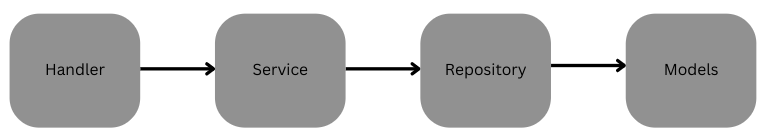
\includegraphics[width=13.8cm, height=2.5cm]{structure_backend.png}

La capa \textbf{Handler} es la encargada de interceptar los requests, interactuar con los permisos, detectar posibles errores dentro del request recibido, preparar las estructuras necesarias para finalmente ejecutar alguno(s) de los servicios de la capa \textbf{Service} para luego retornar el response adecuado para el request.
\newline

La capa \textbf{Service} consta de varios servicios tales como iniciar sesión, registrarse, etc, esta se encarga de ejecutar los pasos necesarios para la acción requerida, abstrayéndose de las validaciones del requests (porque ya fue hecho por la capa \textbf{Handler}), para obtener datos deberá pedírselos a la capa \textbf{Repository} y luego retornarlos a la capa \textbf{Handler}.
\newline

La capa \textbf{Repository} es la encargada de las operaciones con la base de datos, para ello recibe indicaciones de la capa \textbf{Serivice} y auxiliándose del \textit{ORM} \href{gorm.io}{Gorm} y inserta, modifica, lee, y/o elimina datos y le entrega una respuesta a la capa \textbf{Service}.
\newline

La capa \textbf{Models} tiene, con la sintaxis de estructuras de \href{go.dev}{Go}, se describen todas las entidades y las relaciones de la base de datos, para ello hace uso del \textit{ORM} \href{gorm.io}{Gorm}.

\subsection{Usuarios}

\textbf{Crear una cuenta}

Para crear un nuevo usuario se tiene el endpoint de tipo \textbf{POST} a la la url \textit{\textcolor{red}{/api/account/signup}}, el cuerpo de la petición debe tener la siguiente forma:

\begin{lstlisting}[language=javascript]
	{
		"email",
		"name",
		"pass",
		"worker"
	}
\end{lstlisting}

El campo \textit{worker} especifica el rol con el que el usuario va a ser creado inicialmente (que luego puede ser cambiado por el administrador), si se indica que \textit{worker = 0} entonces el rol del usuario será \textbf{estudiante}, de lo contrario será \textbf{clasificador}.
\newline

Luego de validar todos los campos se llama a la función \textit{Signup} del \textit{user\_service}, esta se encarga de encriptar la contraseña para luego llamar a la función \textit{Create} del \textit{user\_repository} cuya tarea es insertar estos datos en la tabla \textit{user}. Para encriptar la contraseña se usa el algoritmo \textit{SHA256} con un salt aleatorio de 32 bits. El salt es guardado junto con la contraseña para poder usarlo a la hora de desencriptarla.
\newline

Luego de esto se genera un token con los datos del usuario usando \textit{JWT} que es devuelto en el response. Este token deberá proveerse en muchos request que requieran autenticación.
\newline

\textbf{Iniciar sesión}

Para iniciar sesión se tiene el endpoint de tipo \textbf{POST} con url \textit{\textcolor{red}{/api/account/signin}}, el cuerpo de la petición debe tener la siguiente forma:

\begin{lstlisting}[language=javascript]
	{
		"email",
		"pass"
	}
\end{lstlisting}

En esta ocasión el handler va a llamar a la función \textit{Signin} de \textit{user\_service}, la cual se va a encargar de encontrar a ese usuario en la base de datos usando la función \textit{FindByEmail} de \textit{user\_repository} y validar la contraseña, si todo está en orden se va a generar un token para retornar en el response.
\newline

\textbf{Crearse una cuenta} e \textbf{iniciar sesión} son las dos únicas operaciones que se pueden hacer sin estar autenticado, en el resto de endpoints se requiere de autenticación, para ello se hace uso del middleware \textit{auth\_user} que verifica si en el header \textit{Authentication} del request hay un token válido, este header debe tener el formato \textit{\textcolor{blue}{Bearer 'token'}}
\newline

\textbf{Middlewares}

A parte del middleware \textit{auth\_user} mencionado anteriormente también se desarrollaron otros 2 que manejan la autorización de un usuario a un recurso dependiendo de su rol:

\begin{lstlisting}[language=go]
	OnlyRoles(roles []string)
\end{lstlisting}

Este middleware recibe un array de strings con los nombres de los roles que deben ser autorizados a acceder al recurso que se quiere proteger.

\begin{lstlisting}[language=go]
	NotTheseRoles(roles []string)
\end{lstlisting}

Por el contrario, este último recibe los nombres de los roles que no deben ser autorizados a determinado recurso que se quiere proteger.
\newline

Se pueden usar indistintamente para la misma función, dependiendo del caso, el primero es más cómodo cuando hay pocos roles a autorizar, y el último casi siempre se usa cuando hay un determinado rol que se quiere desautorizar. 
\newline

\textbf{Modificar rol}

Para modificar el rol de un determinado usuario se creó el endpoint de tipo \textbf{PUT} \textit{\textcolor{red}{/api/users/update-role}}, cuyo cuerpo debe tener la siguiente estructura:

\begin{lstlisting}[language=javascript]
		{
			"user_id"
			"role_id"
		}
\end{lstlisting}

Este endpoint solo puede ser accedido por usuarios con el rol de administrador, y le modifica al usuario con \textit{id = 'user\_id'} su rol al rol con \textit{id = 'role\_id'}